\section{Thiết kế, Hiện thực và Đánh giá}

\subsection{Công nghệ triển khai (Tech Stack)}
Nhằm phát huy tối đa thế mạnh của các thành viên trong nhóm và tính chất của từng dịch vụ, CourtMate được triển khai trên nền tảng công nghệ đa ngôn ngữ (Polyglot Programming):

\begin{itemize}
    \item \textbf{Frontend Application:} Sử dụng Next.js 14 (App Router) kết hợp cùng TailwindCSS, mang lại tốc độ phản hồi nhanh (Server-side Rendering) và giao diện chuẩn UI/UX hiện đại.    \item \textbf{B2C Booking Service:} Xây dựng trên nền tảng Node.js và Express, sử dụng Prisma ORM để tương tác với cơ sở dữ liệu, giúp xử lý các request đặt sân từ người chơi một cách linh hoạt.    \item \textbf{B2B Admin Service:} Sử dụng Java 17 và Spring Boot 3.2 kết hợp cùng Spring Data JPA, đảm bảo tính chặt chẽ và ổn định cho các nghiệp vụ quản lý doanh thu, sân bãi của đối tác.    \item \textbf{AI Pricing Engine:} Triển khai bằng ngôn ngữ Python thông qua framework FastAPI, tận dụng sức mạnh của các thư viện xử lý dữ liệu và máy học chuyên sâu.    \item \textbf{API Documentation:} Sử dụng Swagger/OpenAPI 3.0 để chuẩn hóa tài liệu giao tiếp giữa các dịch vụ B2C, B2B và mã nguồn Frontend.\end{itemize}

\subsection{Đặc tả Giao diện và Trải nghiệm Người dùng}
Tập trung vào các đặc tả kỹ thuật và luồng trải nghiệm người dùng (UX Flow) cho các màn hình cốt lõi của hệ thống CourtMate:

\begin{enumerate}
    \item \textbf{Admin Operational Dashboard}
    \begin{itemize}
        \item \textit{Layout:} Cấu trúc Dashboard tiêu chuẩn với Sidebar menu cố định bên trái, Panel chính bên phải hiển thị các Widget dữ liệu dạng thẻ (Cards).
        \item \textit{Components:} Biểu đồ nhiệt (Heatmap) sử dụng thư viện Recharts để trực quan hóa khung giờ cao điểm; Hệ thống Toast thông báo thời gian thực về các booking mới.
        \item \textit{Flow:} Tự động cập nhật số liệu mỗi [30 giây] qua WebSocket từ Analytics Service; Click vào Widget doanh thu để mở báo cáo chi tiết theo ngày/tuần.
    \end{itemize}

    \item \textbf{Interactive Slot Grid (Quản lý suất chơi)}
    \begin{itemize}
        \item \textit{Layout:} Panel chính hiển thị lưới thời gian (Vertical Axis) và danh sách sân (Horizontal Axis).
        \item \textit{Components:} Drag-and-drop Grid (sử dụng dnd-kit); Hệ thống phân loại màu sắc cho các trạng thái: Trống (Trắng), Đã đặt (Xanh), Đang khóa (Vàng - Pending), Đang xử lý AI (Tím).
        \item \textit{Flow:} Chọn suất chơi trống -> Popup nhanh nhập thông tin khách hàng -> Gọi API Booking Service -> Cập nhật trạng thái sân trên toàn bộ client qua cơ chế Server-Sent Events (SSE) hoặc Short Polling.
    \end{itemize}

    \item \textbf{Spatial Search \& Map View (Tìm kiếm vị trí)}
    \begin{itemize}
        \item \textit{Layout:} Giao diện Split-view; danh sách sân bãi hiển thị bên trái và bản đồ Mapbox chiếm 60\% không gian bên phải.
        \item \textit{Components:} Mapbox GL JS tích hợp Marker Clustering; Bộ lọc đa tầng (vị trí, loại sân, tiện ích, khoảng giá).
        \item \textit{Flow:} Di chuyển bản đồ -> Trigger sự kiện `onMoveEnd` -> Gửi tọa độ Bounding Box về Backend -> Truy vấn Geo-spatial indexing -> Cập nhật danh sách sân bãi tương ứng.
    \end{itemize}

    \item \textbf{Transaction \& Payment Pipeline}
    \begin{itemize}
        \item \textit{Layout:} Quy trình Checkout 3 bước (Thông tin -> Thanh toán -> Xác nhận).
        \item \textit{Components:} Dynamic QR Generator cho MoMo/ZaloPay; Countdown Timer cho cơ chế Khóa suất chơi tạm thời (Optimistic Lock).
        \item \textit{Flow:} Nhấn "Đặt ngay" -> Backend tạo Database-level Optimistic Lock bằng trường \texttt{locked\_until} trong PostgreSQL (TTL 10m) -> Người dùng quét mã QR -> Nhận Webhook từ cổng thanh toán -> Chuyển trạng thái Booking sang CONFIRMED và giải phóng lock.
    \end{itemize}

    \item \textbf{AI Pricing Configurator}
    \begin{itemize}
        \item \textit{Layout:} Giao diện dạng form cấu hình kết hợp biểu đồ dự báo xu hướng.
        \item \textit{Components:} Range Sliders để thiết lập ngưỡng giảm giá (Thresholds); Đồ thị so sánh giá thị trường thời gian thực.
        \item \textit{Flow:} Điều chỉnh tham số đầu vào (ví dụ: Tăng trọng số cho yếu tố thời tiết) -> Preview kết quả giá dự kiến -> Lưu cấu hình xuống AI Engine Service -> AI tự động điều chỉnh giá trên Front-facing app.
    \end{itemize}

    \item \textbf{ERP Integration Sync (MISA)}
    \begin{itemize}
        \item \textit{Layout:} Bảng liệt kê lịch sử đối soát hóa đơn điện tử.
        \item \textit{Components:} Status Badges (Đã đồng bộ, Lỗi, Chờ xử lý); Nút "Manual Sync" cho các trường hợp ngoại lệ.
        \item \textit{Flow:} Transaction xác nhận hoàn tất -> Tự động đẩy dữ liệu sang MISA API -> Nhận mã hóa đơn (UUID) -> Lưu vết và hiển thị trạng thái hóa đơn điện tử cho người chơi.
    \end{itemize}

    \item \textbf{Player Activity Tracker}
    \begin{itemize}
        \item \textit{Layout:} Giao diện Profile cá nhân với hệ thống Milestone và biểu đồ phong độ thể thao.
        \item \textit{Components:} Radar Chart hiển thị kỹ năng; Danh sách thẻ (Cards) hiển thị lịch sử các trận đấu đã tham gia.
        \item \textit{Flow:} Sau mỗi trận đấu, hệ thống tính dựa trên dữ liệu check-in -> Cập nhật điểm tích lũy -> Mở khóa các ưu đãi/vouchers cho các lần đặt sân tiếp theo.
    \end{itemize}

    \item \textbf{Hệ thống Matchmaking (Ghép trận tự động)}
    \begin{itemize}
        \item \textit{Layout:} Giao diện phòng chờ trực quan, hiển thị các trận đấu đang thiếu người dựa trên khoảng cách địa lý.
        \item \textit{Components:} Radar Chart hiển thị kỹ năng; Hệ thống xếp hạng ELO (Competitive Rating).
        \item \textit{Flow:} Người dùng tạo phòng chờ kèm thông số trình độ (Beginner/Intermediate/Advanced) -> Hệ thống Broadcast yêu cầu đến các người chơi phù hợp -> Khi đủ người, tự động tạo Booking và thực hiện chia tiền thanh toán (Split Payment).
    \end{itemize}

    \item \textbf{Recurring Booking (Đặt lịch cố định)}
    \begin{itemize}
        \item \textit{Layout:} Bảng cấu hình lịch biểu tích hợp Calendar view dài hạn.
        \item \textit{Components:} Bulk Slot Checker; Invoice Generator cho hóa đơn tổng.
        \item \textit{Flow:} Chọn khung giờ và khoảng thời gian (VD: 3 tháng) -> Hệ thống kiểm tra xung đột lịch (Conflict Resolution) hàng loạt -> Tạo Bulk Booking và xuất hóa đơn tổng.
    \end{itemize}
\end{enumerate}

\subsection{Luồng hiện thực AI Dynamic Pricing}
Tính năng định giá động được hiện thực hóa thông qua quy trình giao tiếp REST API nội bộ, đảm bảo tính đơn giản và độ tin cậy:

\begin{enumerate}
    \item \textbf{Kích hoạt (Trigger):} Quá trình tính toán được kích hoạt định kỳ bởi hệ thống hoặc thông qua thao tác từ Admin tại B2B Service.
    \item \textbf{Tính toán (AI Computation):} B2B Service thực hiện một cuộc gọi Internal REST API gửi các tham số (vị trí, thời tiết, occupancy) đến AI Engine Service (FastAPI). Tại đây, AI Service thực hiện phân tích rules-based và trả về một Hệ số nhân (Multiplier).
    \item \textbf{Cập nhật (Persistence):} Ngay sau khi nhận kết quả, B2B Service tiến hành một thao tác Bulk Update trực tiếp trường \texttt{slots.price} của các suất chơi tương ứng trong cơ sở dữ liệu PostgreSQL dùng chung.
\end{enumerate}

\subsection{Thiết kế dữ liệu và Thực thể cốt lõi}

\begin{figure}[H]
    \centering
    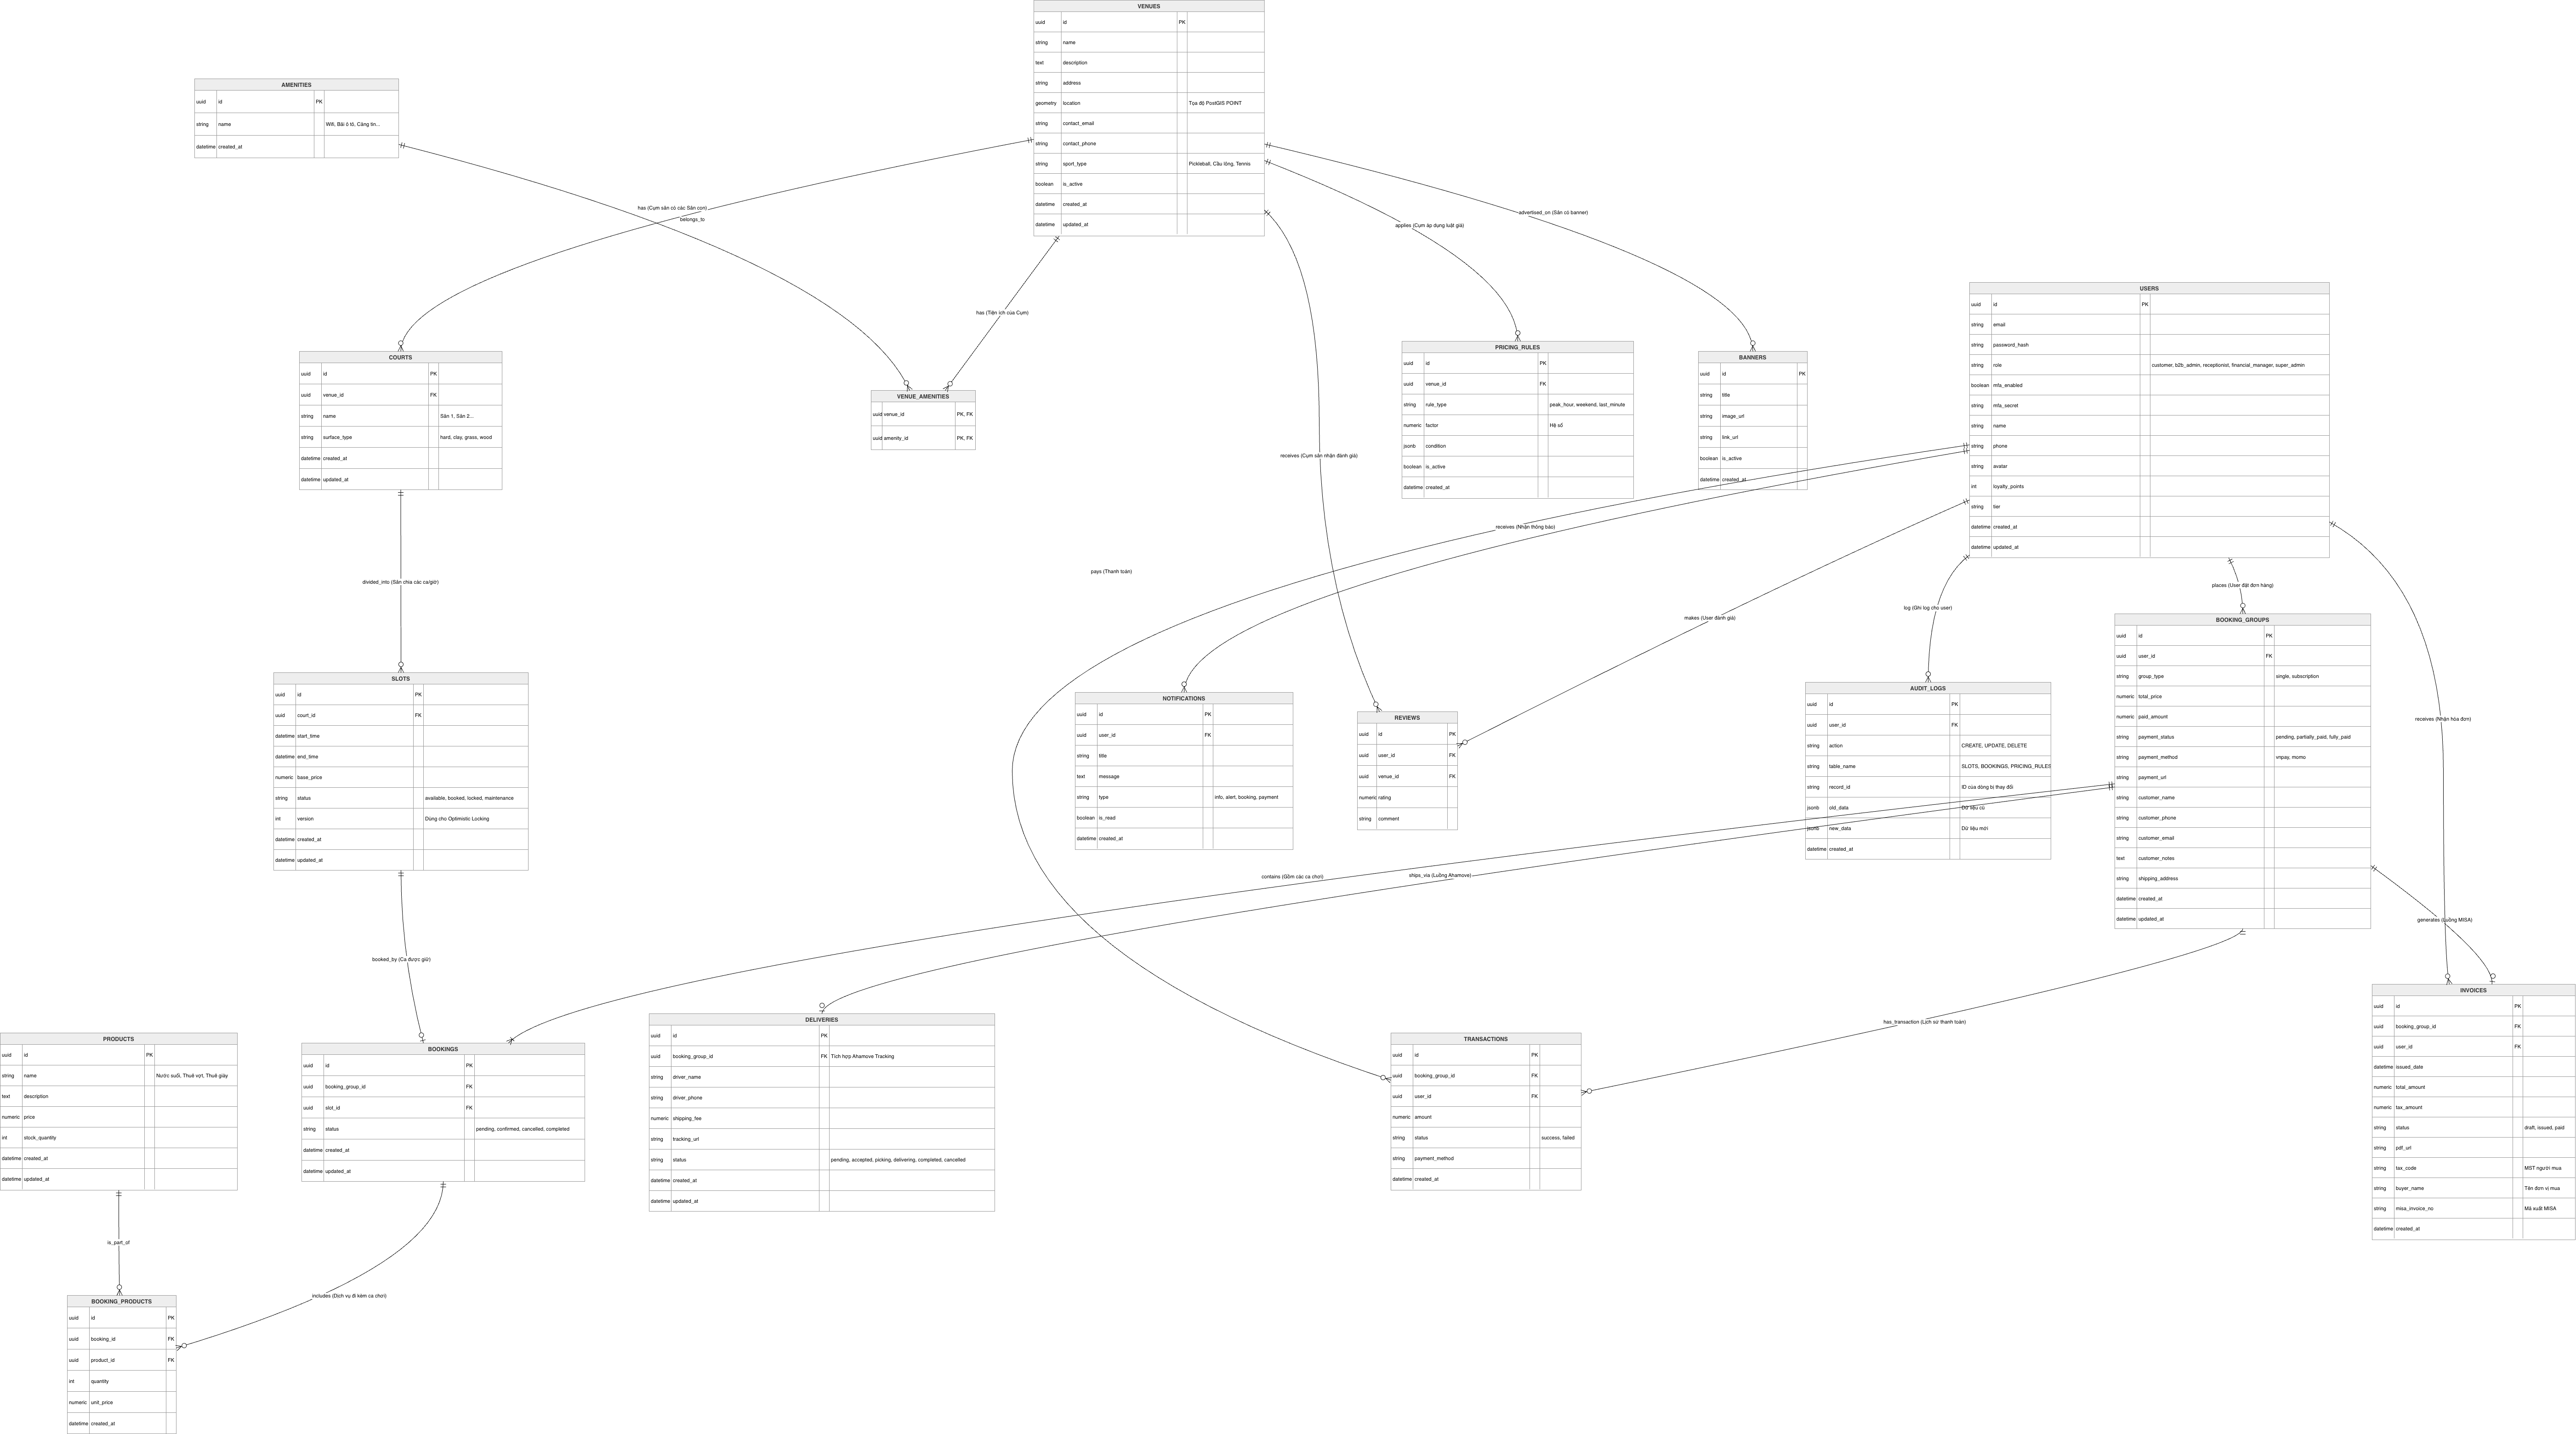
\includegraphics[width=1\textwidth]{Images/eerd.png}
    \caption{Sơ đồ Thực thể - Kết hợp mở rộng (EERD) của hệ thống}
    \label{fig:eerd_diagram}
\end{figure}

Hình \ref{fig:eerd_diagram} trình bày sơ đồ Thực thể - Kết hợp mở rộng (EERD) của hệ thống CourtMate, mô tả cấu trúc dữ liệu cốt lõi và các mối quan hệ giữa các thực thể trong miền nghiệp vụ đặt sân thể thao trực tuyến.

\subsubsection{Chi tiết các thực thể cốt lõi}
Để tối ưu hóa trải nghiệm đọc, các thực thể chính và vai trò của chúng được hệ thống hóa như sau:

\begin{itemize}
    \item \textbf{Bookings (Trung tâm giao dịch):} Lưu trữ toàn bộ thông tin đặt sân. Mỗi booking liên kết với một \textbf{User} và một \textbf{Slot} (quan hệ N:1), cho phép định danh duy nhất và truy vết trạng thái thanh toán, check-in.
    \item \textbf{Slots (Đơn vị suất chơi):} Đại diện cho khung giờ khả dụng. Slots thuộc về \textbf{Court}, và Court thuộc về \textbf{Venue}, tạo nên cấu trúc phân cấp 3 tầng (\textit{Venue $\rightarrow$ Court $\rightarrow$ Slot}).
    \item \textbf{Users (Định danh và Phân quyền):} Hỗ trợ cơ chế Role-based Access Control (RBAC) với các vai trò Player, Owner và Admin, đảm bảo phân tách nghiệp vụ minh bạch giữa B2C và B2B.
\end{itemize}

\subsubsection{Phân nhóm chức năng và Thuộc tính mở rộng}
Hệ thống tổ chức dữ liệu theo các nhóm chức năng độc lập nhằm đảm bảo tính mô-đun (modularity):

\begin{description}
    \item[Nhóm Vận hành thời gian thực:] Bao gồm các thuộc tính như \texttt{status} (available, locked, booked) và \texttt{locked\_until} để hiện thực hóa cơ chế \textit{Optimistic Locking}, chống tình trạng Overbooking.
    \item[Nhóm Tài chính và Hậu cần:] Liên kết giữa \textbf{Bookings} với các thực thể \textbf{Payments}, \textbf{Transactions} và \textbf{Invoices} (Hóa đơn điện tử), hỗ trợ đối soát tự động và tích hợp MISA.
    \item[Nhóm Tương tác và Mở rộng:] Các thực thể \textbf{Reviews} (đánh giá), \textbf{Matchmaking} (ghép trận) và cấu hình \textbf{Pricing} (định giá động) được thiết kế tách biệt để có thể nâng cấp mà không ảnh hưởng đến lõi hệ thống.
\end{description}

Thiết kế dữ liệu theo hướng chuẩn hóa kết hợp với \textbf{Shared Database Pattern} giúp giảm thiểu dư thừa dữ liệu, đồng thời đảm bảo khả năng thực thi các truy vấn Join hiệu quả phục vụ báo cáo doanh thu và phân tích hành vi người dùng.

\subsection{Đánh giá Hiệu năng và Độ ổn định}
Do hệ thống đã được tối giản hóa về mặt kiến trúc, trọng tâm của việc đánh giá được đặt vào tính chính xác của nghiệp vụ và khả năng chịu tải ở mức trung bình của Shared Database. Các bài kiểm tra nội bộ cho thấy hệ thống vận hành trơn tru với cấu hình hạ tầng hiện tại, phản hồi các truy vấn tìm kiếm và đặt sân trong thời gian chấp nhận được đối với một ứng dụng web thương mại điện tử.

\subsection{Kế hoạch quản lý rủi ro hệ thống}
Để đảm bảo tính bền vững và độ tin cậy của CourtMate, nhóm đã thiết lập khung quản lý rủi ro tập trung vào các đặc thù của kiến trúc Microservices và mô hình Shared Database:

\begin{table}[H]
    \centering
    \renewcommand{\arraystretch}{1.3}
    \begin{tabularx}{\textwidth}{|c|p{3.5cm}|c|X|}
    \hline
    \textbf{STT} & \textbf{Tên rủi ro} & \textbf{Mức độ} & \textbf{Chiến lược phòng ngừa \& giải quyết} \\ \hline
    1 & Quá tải Shared Database khi test tải cực đại & Cao & Tối ưu hóa Database Indexing, sử dụng Connection Pooling và thiết lập Resource Limits cho mỗi service truy cập. \\ \hline
    2 & Trễ tiến độ tích hợp API bên thứ 3 (MoMo, MISA) & Trung bình & Xây dựng Adapter Service với cơ chế Retry logic và Circuit Breaker; sử dụng Mock API trong giai đoạn phát triển. \\ \hline
    3 & Vượt ngân sách hạ tầng Cloud (Free Tier) & Thấp & Thiết lập Budget Alerts trên AWS/GCP; tối ưu kích thước Docker Image và tắt các service không thiết yếu khi không demo. \\ \hline
    4 & Lỗi Race Condition dẫn đến Overbooking & Cao & Áp dụng Database-level Optimistic Lock qua trường \texttt{locked\_until} hoặc versioning trong các transaction thanh toán. \\ \hline
    \end{tabularx}
    \caption{Bảng kế hoạch quản lý rủi ro hệ thống CourtMate}
    \label{tab:risk_management}
\end{table}

